\providecommand{\rasd}{..}
\documentclass[../RASD.tex]{subfiles}

\begin{document}
    \chapter{Formal analysis using alloy }\label{ch:formal-analysis-using-alloy}
    This section presents a possible Alloy formalization of the proposed system.
    This Alloy model illustrates the key concepts and entities that make up the system and the relationships
    between them, and is to be seen as an attempt of capturing the systems essential features.
    This model has the purpose of verifying if the properties defined for the system are possible to satisfy and if there are no constraints being violated.
    Although this model is a simplified version of the real world, it is enough to show that the model stands in the scope of the project.

    \section{Alloy Model}\label{sec:alloy-model}
        \vspace{2 mm}
        \lstinputlisting[language=alloy]{
        formal_analysis_using_alloy/alloy.als
        }
        \vspace{8 mm}

    \section{Generated World}\label{sec:generated-world}
    After running the model described above, different worlds were generated.
    Because of simplicity, strings and integers have not been distinguished for different contexts.
    Even if this could seems an excessive simplification, it is actually a possible situation, since some data could be the same for different contexts.
    \begin{figure}[H]
        \centering
        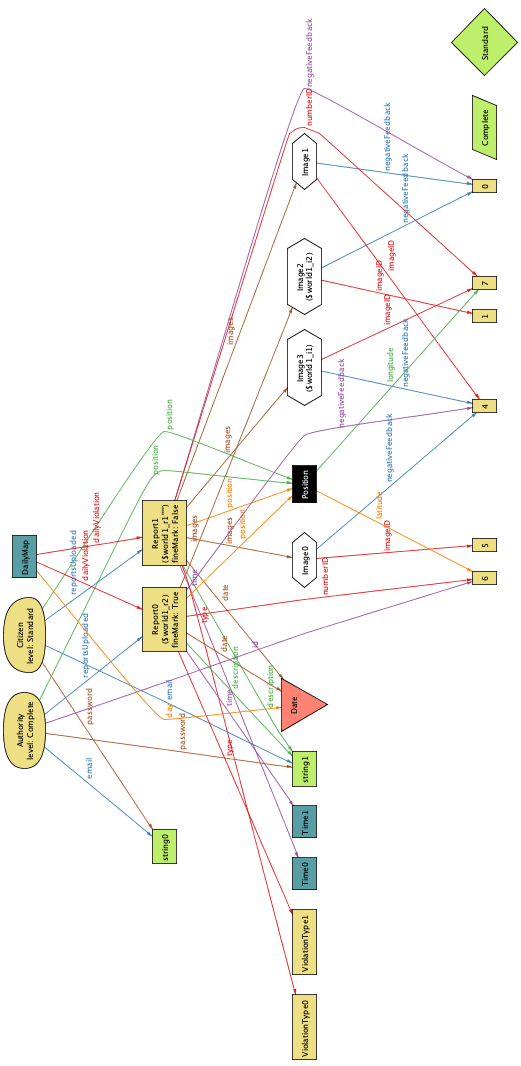
\includegraphics[scale = 0.7]{assets/world1.png}\\
        \caption[Generated world 1, \textit{Alloy}]{Generated world 1, \textit{Alloy}}
    \end{figure}

    From the first world generated we can see that every report must belong to a user.
    Every report must contains all the mandatory information: violation type, location, date, time, user itself and the images are correctly generated.
    Moreover, we can see the each report can contains more than one picture.

    \begin{figure}[H]
        \centering
        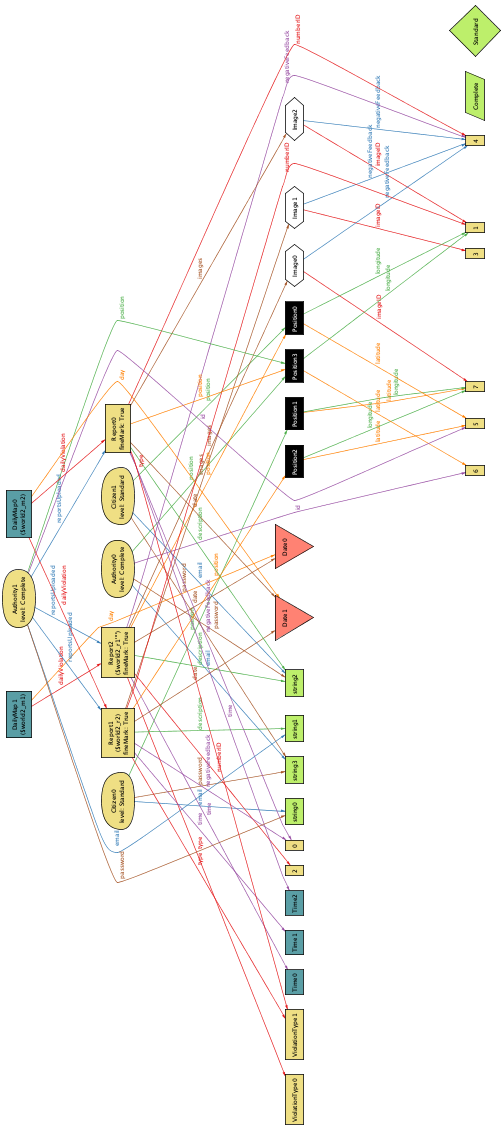
\includegraphics[scale = 0.6]{assets/world2.png}\\
        \caption[Generated world 2, \textit{Alloy}]{Generated world 2, \textit{Alloy}}
    \end{figure}

    In this second world is showed the important correspondence between a daily violation map and its report:
    it is possible to notice that all the report are assigned to the daily map that correspond to their upload date (it may be useful to remember that the upload date is the actually date of the violation, since the report must be uploaded in real time)

    \begin{figure}[H]
        \centering
        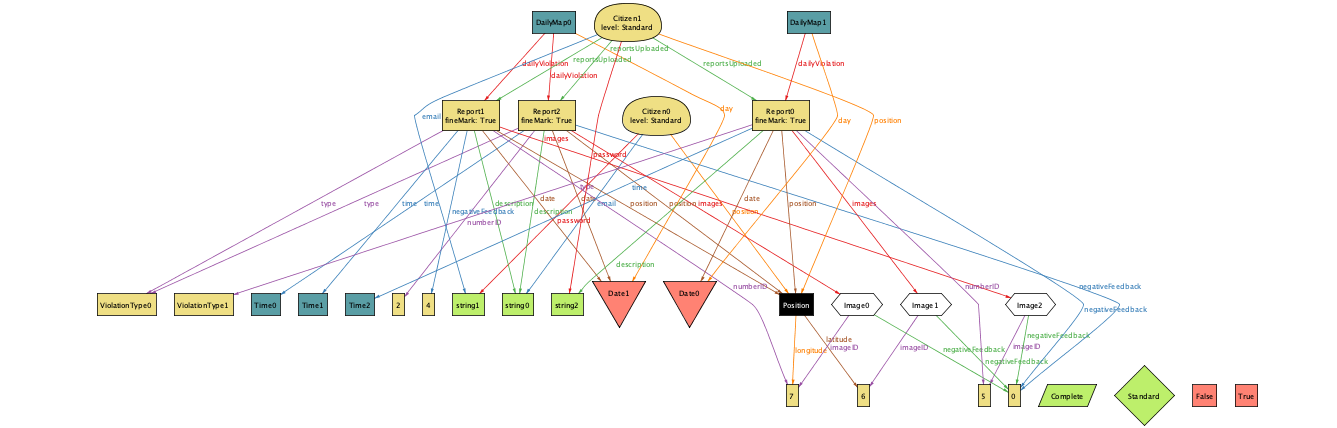
\includegraphics[scale = 0.7]{assets/world3.png}\\
        \caption[Generated world 3, \textit{Alloy}]{Generated world 3, \textit{Alloy}}
    \end{figure}

    In this last picture, we can see a generic representation of the system.
    It has been generated with no constrains, and it is possible to notice that it is consistent with all the assumption done in this document.

\end{document}